\documentclass[11pt,a4paper]{article}

\usepackage[utf8]{inputenc}
\usepackage[T1]{fontenc}
\usepackage[spanish,es-nodecimaldot]{babel}
\usepackage{geometry}
\usepackage{amsmath}
\usepackage{amssymb}
\usepackage{booktabs}
\usepackage{array}
\usepackage{graphicx}
\usepackage{float}
\usepackage{hyperref}
\usepackage{tabularx}
\usepackage{enumitem}
\usepackage{xcolor}
\usepackage{caption}
\usepackage{natbib}
\usepackage{multirow}
\usepackage{url}

\geometry{margin=2.5cm}
\emergencystretch=1.5em
\hypersetup{
    colorlinks=true,
    linkcolor=blue!50!black,
    citecolor=blue!50!black,
    urlcolor=blue!50!black,
    pdftitle={Informe tecnico de la intervencion Markoviana para TD3 en protesis mioelectrica},
    pdfauthor={Proyecto EMG\_Prosthesis\_TD3}
}

\newcolumntype{L}[1]{>{\raggedright\arraybackslash}p{#1}}
\newcolumntype{C}[1]{>{\centering\arraybackslash}p{#1}}
\newcolumntype{Y}{>{\raggedright\arraybackslash}X}

\title{\textbf{Informe T\'ecnico Mejorado de la Intervenci\'on Markoviana}\\
\large TD3 para control continuo de pr\'otesis mioel\'ectrica en simulaci\'on}
\author{Proyecto \texttt{EMG\_Prosthesis\_TD3}}
\date{19 de marzo de 2026}

\begin{document}

\maketitle

\begin{abstract}
Este informe documenta la intervenci\'on m\'as reciente aplicada al proyecto de control continuo de pr\'otesis mioel\'ectrica con TD3 en MATLAB. El foco ya no est\'a en la correcci\'on b\'asica de la reward o en la autoridad de control, sino en mejorar la consistencia Markoviana del entorno y la calidad de la pol\'itica aprendida. La intervenci\'on nueva introduce un estado ampliado de 52 dimensiones, que incorpora deltas de encoder y la acci\'on efectiva previa, y reemplaza la reward con historia oculta por una reward observable-consistente basada en tracking MSE, magnitud de acci\'on y cambio de acci\'on. El entrenamiento reciente de 2000 episodios muestra el mejor \texttt{trackingMSE} medio observado hasta ahora en entrenamiento (\(0.1055\)), pero el test del \texttt{Agent2000} indica que la mejora en tracking final es todav\'ia marginal. Sin embargo, la nueva formulaci\'on s\'i reduce de forma clara la agresividad del control en evaluaci\'on: frente al test de la etapa anterior, el \texttt{actionL2} disminuye \(\approx 32\%\), la fracci\'on de saturaci\'on \(\approx 57\%\) y \(\Delta a\) L2 \(\approx 64\%\), manteniendo el \texttt{trackingMSE} pr\'acticamente igual. La conclusi\'on central es que la intervenci\'on Markoviana mejor\'o la calidad del comportamiento aprendido, pero a\'un no resuelve el seguimiento fino de la referencia; el siguiente trabajo debe orientarse a selecci\'on de checkpoints, auditor\'ia cuantitativa completa y enriquecimiento temporal de la informaci\'on EMG antes de considerar hardware.
\end{abstract}

\section{Objetivo de este informe}

El objetivo de este documento es dejar una versi\'on m\'as clara y profunda del estado actual del proyecto, con \'enfasis en la \textbf{intervenci\'on Markoviana reciente}. El documento resume brevemente las etapas previas, explica con detalle el porqu\'e de los cambios nuevos, formaliza matem\'aticamente el estado y la reward actual, presenta los resultados del entrenamiento de 2000 episodios y del test posterior, y deja una interpretaci\'on t\'ecnica fundamentada sobre qu\'e mejor\'o, qu\'e no mejor\'o y qu\'e deber\'ia cambiarse despu\'es.

Todo el an\'alisis descrito aqu\'i corresponde exclusivamente a \textbf{simulaci\'on con datos preregistrados}, con:
\begin{itemize}[leftmargin=1.2cm]
    \item \texttt{usePrerecorded = true},
    \item \texttt{simMotors = true},
    \item \texttt{connect\_glove = false}.
\end{itemize}
No se ha usado hardware real en ninguna de las corridas documentadas en esta versi\'on del trabajo.

\section{Antecedentes breves y \'utiles}

Las etapas previas siguen siendo relevantes, pero aqu\'i solo se resumen sus hallazgos esenciales para contextualizar la intervenci\'on nueva. La Tabla~\ref{tab:history} sintetiza esa evoluci\'on.

\begin{table}[H]
\centering
\caption{Resumen breve de las etapas previas}
\label{tab:history}
\small
\setlength{\tabcolsep}{5pt}
\renewcommand{\arraystretch}{1.15}
\begin{tabularx}{\textwidth}{L{0.18\textwidth}L{0.24\textwidth}Y Y}
\toprule
\textbf{Etapa} & \textbf{Cambio principal} & \textbf{Aporte \'util} & \textbf{L\'imite detectado} \\
\midrule
Legacy 50 & Reward heredada discreta y entorno original & Sirvi\'o como baseline de referencia muy temprana. & Reward incoherente con TD3 continuo, poca trazabilidad y se\~nal dif\'icil de interpretar. \\
MSE coherente 300 & Reward densa basada en tracking MSE normalizado y regularizaci\'on de acci\'on & Volvi\'o el entrenamiento auditable; aline\'o la reward con tracking real; corrigi\'o el \texttt{step}. & El agente segu\'ia siendo conservador y no explotaba bien la acci\'on en el simulador. \\
Remapeo 5000 & Remapeo expl\'icito a PWM efectivo y compensaci\'on de zona muerta & Corrigi\'o una incoherencia f\'isica real entre acci\'on continua y actuaci\'on aplicada. & M\'as autoridad de control no produjo una mejora clara de tracking; aparecieron pol\'iticas agresivas. \\
Progreso + suavidad 3000 & Reward con progreso temporal y penalizaci\'on de cambio de acci\'on & Baj\'o parcialmente la agresividad media en entrenamiento. & La reward depend\'ia de historia no observada por el actor; el test no mejor\'o tracking y segu\'ia habiendo colapso parcial hacia pol\'iticas pobres. \\
\bottomrule
\end{tabularx}
\normalsize
\end{table}

La lectura t\'ecnica de estas etapas fue la siguiente:
\begin{enumerate}[leftmargin=1.2cm]
    \item primero era necesario sanear el experimento para que reward, entorno y TD3 fueran interpretables;
    \item luego fue necesario hacer que la acci\'on continua del actor tuviera efecto f\'isico real en simulaci\'on;
    \item finalmente apareci\'o el problema actual: el agente \emph{s\'i act\'ua}, pero no usa esa acci\'on con la coordinaci\'on suficiente para mejorar tracking.
\end{enumerate}

La corrida larga de 5000 episodios de la etapa de remapeo fue la que dej\'o m\'as clara esa transici\'on. Su curva se incluye en la Figura~\ref{fig:train5000}, porque es el punto en el que el problema dej\'o de ser ``falta de acci\'on efectiva'' y pas\'o a ser ``calidad de pol\'itica''.

\IfFileExists{figures/5000pro.png}{
\begin{figure}[H]
\centering
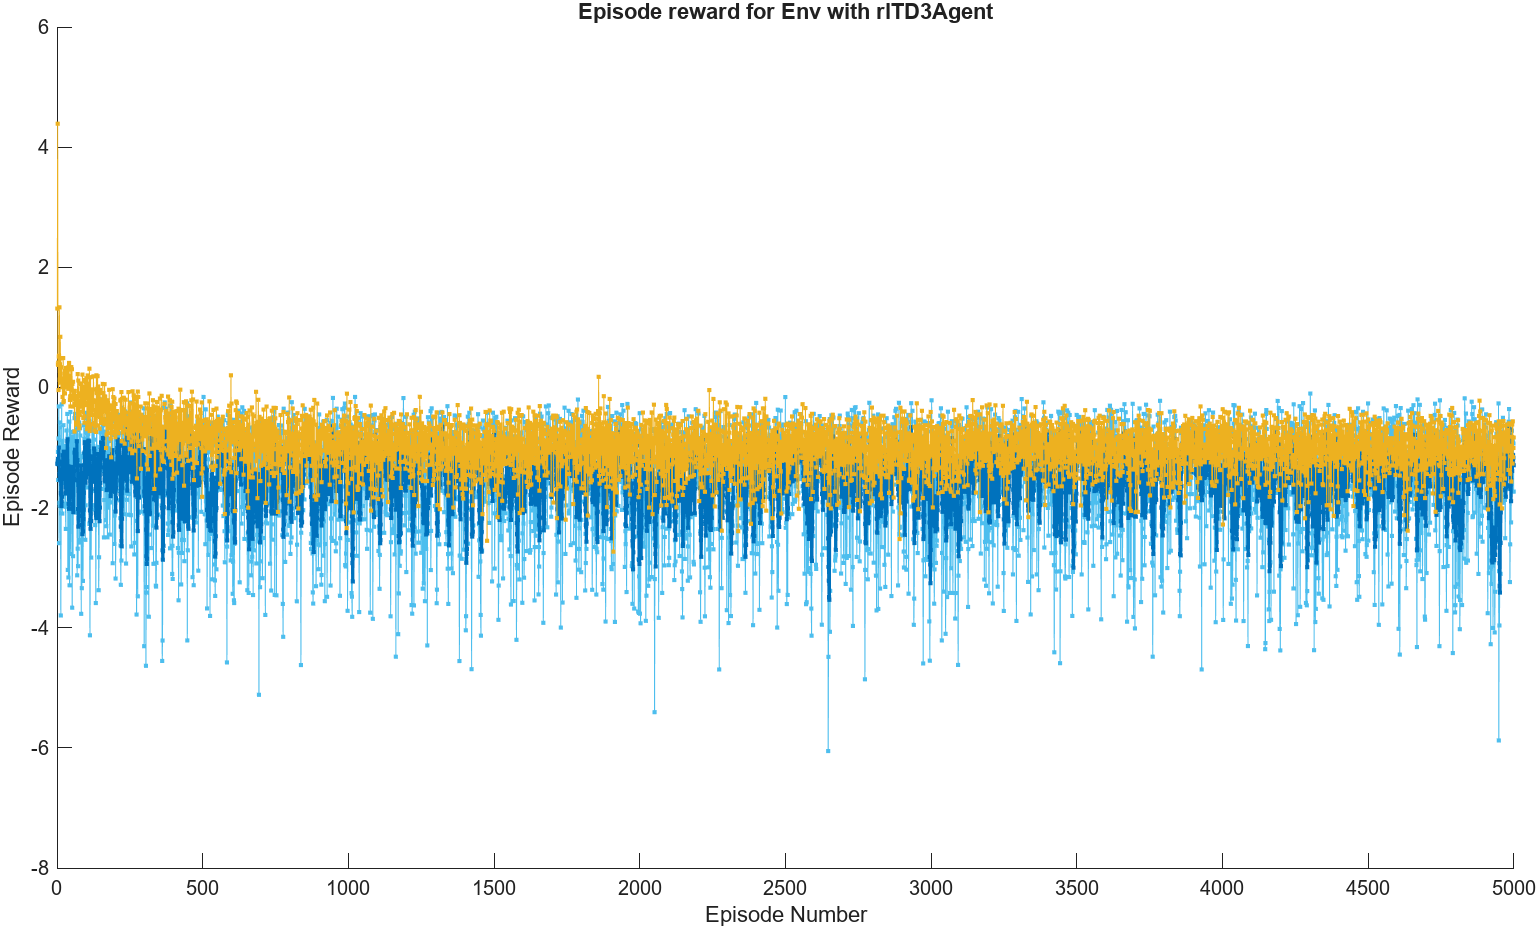
\includegraphics[width=\textwidth]{figures/5000pro.png}
\caption{Corrida larga de 5000 episodios con remapeo de acci\'on efectiva. La mejora del tracking se estanca, aunque la acci\'on aplicada aumenta.}
\label{fig:train5000}
\end{figure}
}{}

En esa corrida, el \texttt{trackingMSE} medio qued\'o en \(0.1070\), mientras el esfuerzo de control subi\'o de forma clara (\texttt{actionL2} medio \(= 0.3108\), \(|PWM|\) medio \(= 125.06\)). El hallazgo principal fue que \textbf{hacer m\'as fuerte la acci\'on no bastaba}.

\section{Motivaci\'on de la nueva intervenci\'on}

La intervenci\'on actual nace de un diagn\'ostico puntual del dise\~no previo. En la etapa \emph{progreso+suavidad}, la reward depend\'ia de:
\begin{itemize}[leftmargin=1.2cm]
    \item la acci\'on previa \(\tilde{a}_{t-1}\),
    \item el \texttt{trackingMSE} previo.
\end{itemize}
Sin embargo, el estado observado por el actor segu\'ia teniendo solo 44 dimensiones:
\[
s_t^{(44)} =
\begin{bmatrix}
\phi(\mathrm{EMG}_t) \\
\mathrm{enc}_t
\end{bmatrix},
\]
es decir, 40 caracter\'isticas EMG y 4 encoders normalizados.

Ese dise\~no introduc\'ia una asimetr\'ia importante: la reward usaba historia reciente que el actor no ve\'ia de forma expl\'icita. En t\'erminos de dise\~no de entorno, esto no romp\'ia la implementaci\'on de MATLAB, pero s\'i deterioraba la consistencia pr\'actica del problema para una pol\'itica determinista. Dado que TD3 asume una relaci\'on estable entre observaci\'on, acci\'on y retorno futuro \citep{fujimoto2018td3,mathworks_td3_agent}, mantener historia relevante fuera de la observaci\'on pod\'ia inducir un comportamiento parcialmente observable sin compensaci\'on arquitect\'onica.

Adem\'as, desde el punto de vista de control mioel\'ectrico, la informaci\'on temporal no es un detalle secundario. Las revisiones recientes sobre control mioel\'ectrico subrayan que la din\'amica temporal de la se\~nal y el contexto secuencial son determinantes para controlar m\'ultiples grados de libertad de manera estable \citep{chen2023review}. Del mismo modo, en rob\'otica RL se ha mostrado que regularizar suavidad ayuda, pero su efecto depende de que la pol\'itica tenga suficiente contexto para interpretar el cambio de acci\'on \citep{lee2024smoothness}. En manipulaci\'on rob\'otica tambi\'en existe evidencia de que condicionar la pol\'itica con acci\'on previa o informaci\'on temporal mejora el comportamiento secuencial \citep{kumra2022pacromannet}.

Por eso la nueva intervenci\'on persigui\'o dos objetivos muy concretos:
\begin{enumerate}[leftmargin=1.2cm]
    \item hacer el problema \textbf{m\'as Markoviano} para TD3;
    \item simplificar la reward para que toda la historia usada por la penalizaci\'on estuviera disponible para el agente.
\end{enumerate}

\section{Formulaci\'on t\'ecnica actual}

\subsection{Acci\'on efectiva retenida desde la etapa anterior}

La intervenci\'on nueva no deshizo el remapeo de acci\'on efectiva. Ese cambio se mantuvo porque era f\'isicamente correcto y resolv\'ia un problema real del simulador. La acci\'on continua del actor \(a_t \in [-1,1]^4\) sigue convirti\'endose en una acci\'on efectiva \(\tilde{a}_t\) mediante cuantizaci\'on de PWM:
\begin{equation}
u_{t,i}^{\mathrm{eff}} =
\begin{cases}
0, & |a_{t,i}| < \epsilon, \\
\mathrm{sign}(a_{t,i})\, q\!\left(255|a_{t,i}|\right), & |a_{t,i}| \ge \epsilon,
\end{cases}
\label{eq:effective_pwm_new}
\end{equation}
donde:
\begin{itemize}[leftmargin=1.2cm]
    \item \(\epsilon = 0.05\),
    \item \(q(\cdot)\) cuantiza a los niveles \(\{64, 96, 128, 160, 192, 224, 255\}\),
    \item \(\tilde{a}_{t,i} = u_{t,i}^{\mathrm{eff}} / 255\).
\end{itemize}

Este remapeo sigue siendo necesario porque el simulador y la conversi\'on encoder--flex no responden de manera lineal a acciones continuas peque\~nas. En otras palabras, no es correcto entrenar como si el actuador ejecutara exactamente la salida continua del actor; por eso la reward y el estado usan la acci\'on \emph{efectiva} y no la acci\'on \emph{cruda}.

\subsection{Nuevo estado de 52 dimensiones}

El nuevo estado se defini\'o como:
\begin{equation}
s_t =
\begin{bmatrix}
\phi(\mathrm{EMG}_t) \\
\mathrm{enc}_t \\
\Delta \mathrm{enc}_t \\
\tilde{a}_{t-1}
\end{bmatrix}
\in \mathbb{R}^{52},
\label{eq:state52}
\end{equation}
donde:
\begin{align}
\phi(\mathrm{EMG}_t) &\in \mathbb{R}^{40}, \\
\mathrm{enc}_t &\in \mathbb{R}^{4}, \\
\Delta \mathrm{enc}_t &= \mathrm{enc}_t - \mathrm{enc}_{t-1} \in [-1,1]^4, \\
\tilde{a}_{t-1} &\in [-1,1]^4.
\end{align}

La Tabla~\ref{tab:state52} resume el significado funcional de cada bloque.

\begin{table}[H]
\centering
\caption{Estructura del nuevo estado de 52 dimensiones}
\label{tab:state52}
\small
\setlength{\tabcolsep}{5pt}
\renewcommand{\arraystretch}{1.15}
\begin{tabularx}{\textwidth}{L{0.22\textwidth}C{0.10\textwidth}L{0.20\textwidth}Y}
\toprule
\textbf{Bloque} & \textbf{Dim.} & \textbf{Fuente} & \textbf{Prop\'osito} \\
\midrule
\(\phi(\mathrm{EMG}_t)\) & 40 & \texttt{getWmoosFeatures} & Mantener la base de inferencia mioel\'ectrica original. \\
\(\mathrm{enc}_t\) & 4 & Encoders normalizados & Informar la postura actual de la pr\'otesis. \\
\(\Delta \mathrm{enc}_t\) & 4 & Diferencia de encoders normalizados & Hacer visible el efecto reciente del movimiento y dar contexto din\'amico m\'inimo. \\
\(\tilde{a}_{t-1}\) & 4 & Acci\'on efectiva previa & Hacer observable la historia inmediata relevante para suavidad y coordinaci\'on secuencial. \\
\bottomrule
\end{tabularx}
\normalsize
\end{table}

La idea no fue introducir una memoria grande ni una arquitectura recurrente. La intervenci\'on busc\'o un cambio \emph{m\'inimo y atribuible}: si el problema era la falta de contexto temporal inmediato, entonces bastaba con exponer al actor el \emph{efecto reciente} de la din\'amica y la \emph{acci\'on previa realmente aplicada}.

\subsection{Reward simplificada y observable-consistente}

La reward nueva elimina el t\'ermino de progreso basado en \(\mathrm{MSE}_{t-1}\), precisamente porque ese valor previo no era parte del estado. La formulaci\'on actual es:
\begin{equation}
r_t =
-\frac{1}{4}\sum_{i=1}^{4}
\left(
e_{t,i}^2 +
\lambda_a \tilde{a}_{t,i}^2 +
\lambda_{\Delta a}\left(\tilde{a}_{t,i} - \tilde{a}_{t-1,i}\right)^2
\right),
\label{eq:reward_markov}
\end{equation}
con:
\begin{equation}
e_{t,i} = \hat{y}_{t,i} - y_{t,i}^{\star},
\end{equation}
donde \(\hat{y}_{t,i}\) es la flex estimada de la pr\'otesis y \(y_{t,i}^{\star}\) es la flex de referencia proveniente del glove en simulaci\'on.

Los pesos usados en esta etapa fueron:
\begin{equation}
\lambda_a = 0.01,
\qquad
\lambda_{\Delta a} = 0.05.
\label{eq:reward_weights}
\end{equation}

Esta reward conserva tres propiedades importantes:
\begin{enumerate}[leftmargin=1.2cm]
    \item el t\'ermino principal sigue siendo tracking MSE, que ya hab\'ia mostrado coherencia con el objetivo del proyecto;
    \item la penalizaci\'on de magnitud de acci\'on se aplica sobre la acci\'on \emph{efectiva} y no sobre la acci\'on idealizada;
    \item la penalizaci\'on de cambio de acci\'on se mantiene, pero ahora el agente s\'i observa \(\tilde{a}_{t-1}\), por lo que la reward deja de depender de historia oculta.
\end{enumerate}

Desde la literatura, esta decisi\'on es coherente con dos l\'ineas: reward shaping denso para manipulaci\'on y regularizaci\'on de suavidad para evitar cambios bruscos \citep{deng2025reward,lee2024smoothness}. En nuestro caso, la contribuci\'on pr\'actica fue \textbf{simplificar la reward y trasladar la memoria relevante al estado}.

\subsection{Hiperpar\'ametros TD3 mantenidos}

La intervenci\'on no cambi\'o el algoritmo ni la arquitectura base del agente. Se mantuvo TD3 con la misma MLP, porque el diagn\'ostico actual no apunta a un fallo de implementaci\'on del algoritmo, sino a un problema de representaci\'on del estado y de dise\~no de reward. La Tabla~\ref{tab:td3hparams} resume la configuraci\'on actual.

\begin{table}[H]
\centering
\caption{Hiperpar\'ametros TD3 mantenidos en la intervenci\'on Markoviana}
\label{tab:td3hparams}
\small
\setlength{\tabcolsep}{5pt}
\renewcommand{\arraystretch}{1.15}
\begin{tabularx}{\textwidth}{L{0.30\textwidth}C{0.15\textwidth}Y}
\toprule
\textbf{Par\'ametro} & \textbf{Valor} & \textbf{Rol t\'ecnico} \\
\midrule
Unidades ocultas actor/cr\'iticos & 64 & Capacidad moderada, suficiente para esta escala sin aumentar demasiado el costo de entrenamiento. \\
Actor learning rate & \(1\times10^{-4}\) & Mantiene actualizaciones conservadoras de la pol\'itica. \\
Critic learning rate & \(1\times10^{-3}\) & Permite que el cr\'itico se adapte m\'as r\'apido que el actor. \\
L2 regularization & \(1\times10^{-4}\) & Ayuda a evitar pesos excesivos y estabiliza la optimizaci\'on. \\
Gradient threshold & 1 & L\'imite pr\'actico frente a gradientes extremos. \\
Target smooth factor & 0.005 & Actualizaci\'on lenta de redes objetivo, acorde a TD3 \citep{mathworks_td3_options}. \\
Discount factor \(\gamma\) & 0.95 & Horizonte razonable para episodios cortos de \(\approx 14\) pasos. \\
Mini-batch size & 128 & Compromiso entre ruido de gradiente y costo de c\'omputo. \\
Replay buffer & \(10^5\) & Escala adecuada para corridas largas en este problema. \\
Policy update frequency & 2 & Implementa \textit{delayed policy updates}, uno de los n\'ucleos de TD3 \citep{fujimoto2018td3}. \\
Target update frequency & 2 & Sincroniza redes objetivo con la estrategia de actualizaci\'on diferida. \\
Exploration std & 0.2 & Exploraci\'on continua moderada durante entrenamiento. \\
Exploration std min & 0.02 & Evita que la exploraci\'on colapse completamente. \\
Target policy std & 0.2 & Suavizado de la pol\'itica objetivo para reducir errores por sobreestimaci\'on \citep{fujimoto2018td3}. \\
Target policy clip & 0.5 & Limita el ruido objetivo para evitar perturbaciones excesivas. \\
\bottomrule
\end{tabularx}
\normalsize
\end{table}

\section{Protocolo experimental de la etapa actual}

El piloto nuevo se entren\'o desde cero con:
\begin{itemize}[leftmargin=1.2cm]
    \item reward \texttt{trackingMseActionRateReward},
    \item estado de 52 dimensiones,
    \item 2000 episodios,
    \item guardado cada 50 episodios,
    \item sin plots de entrenamiento en vivo,
    \item simulaci\'on pura con dataset preregistrado.
\end{itemize}

La corrida qued\'o almacenada en:
\[
\texttt{26-03-19 02 26 41}.
\]

Despu\'es del entrenamiento se ejecut\'o un test visual y cuantitativo del checkpoint final:
\[
\texttt{Agent2000.mat},
\]
con 50 simulaciones y generaci\'on de figuras de episodio. El directorio de test correspondiente fue:
\[
\texttt{26-03-19 05 25 26}.
\]

Es importante notar que el checkpoint evaluado fue el final nominal de la corrida, no necesariamente el mejor checkpoint global. Esto se hizo para cerrar una primera evaluaci\'on end-to-end de la intervenci\'on nueva. El mejor promedio de reward de entrenamiento ocurri\'o alrededor del episodio 1892, de modo que una auditor\'ia fina de checkpoints (\texttt{Agent1850}, \texttt{Agent1900}, \texttt{Agent1950}, \texttt{Agent2000}) sigue siendo una tarea pendiente y necesaria.

\section{Resultados cuantitativos}

\subsection{Corrida nueva de 2000 episodios}

\IfFileExists{figures/training_progress_2000eps_markov.png}{
\begin{figure}[H]
\centering
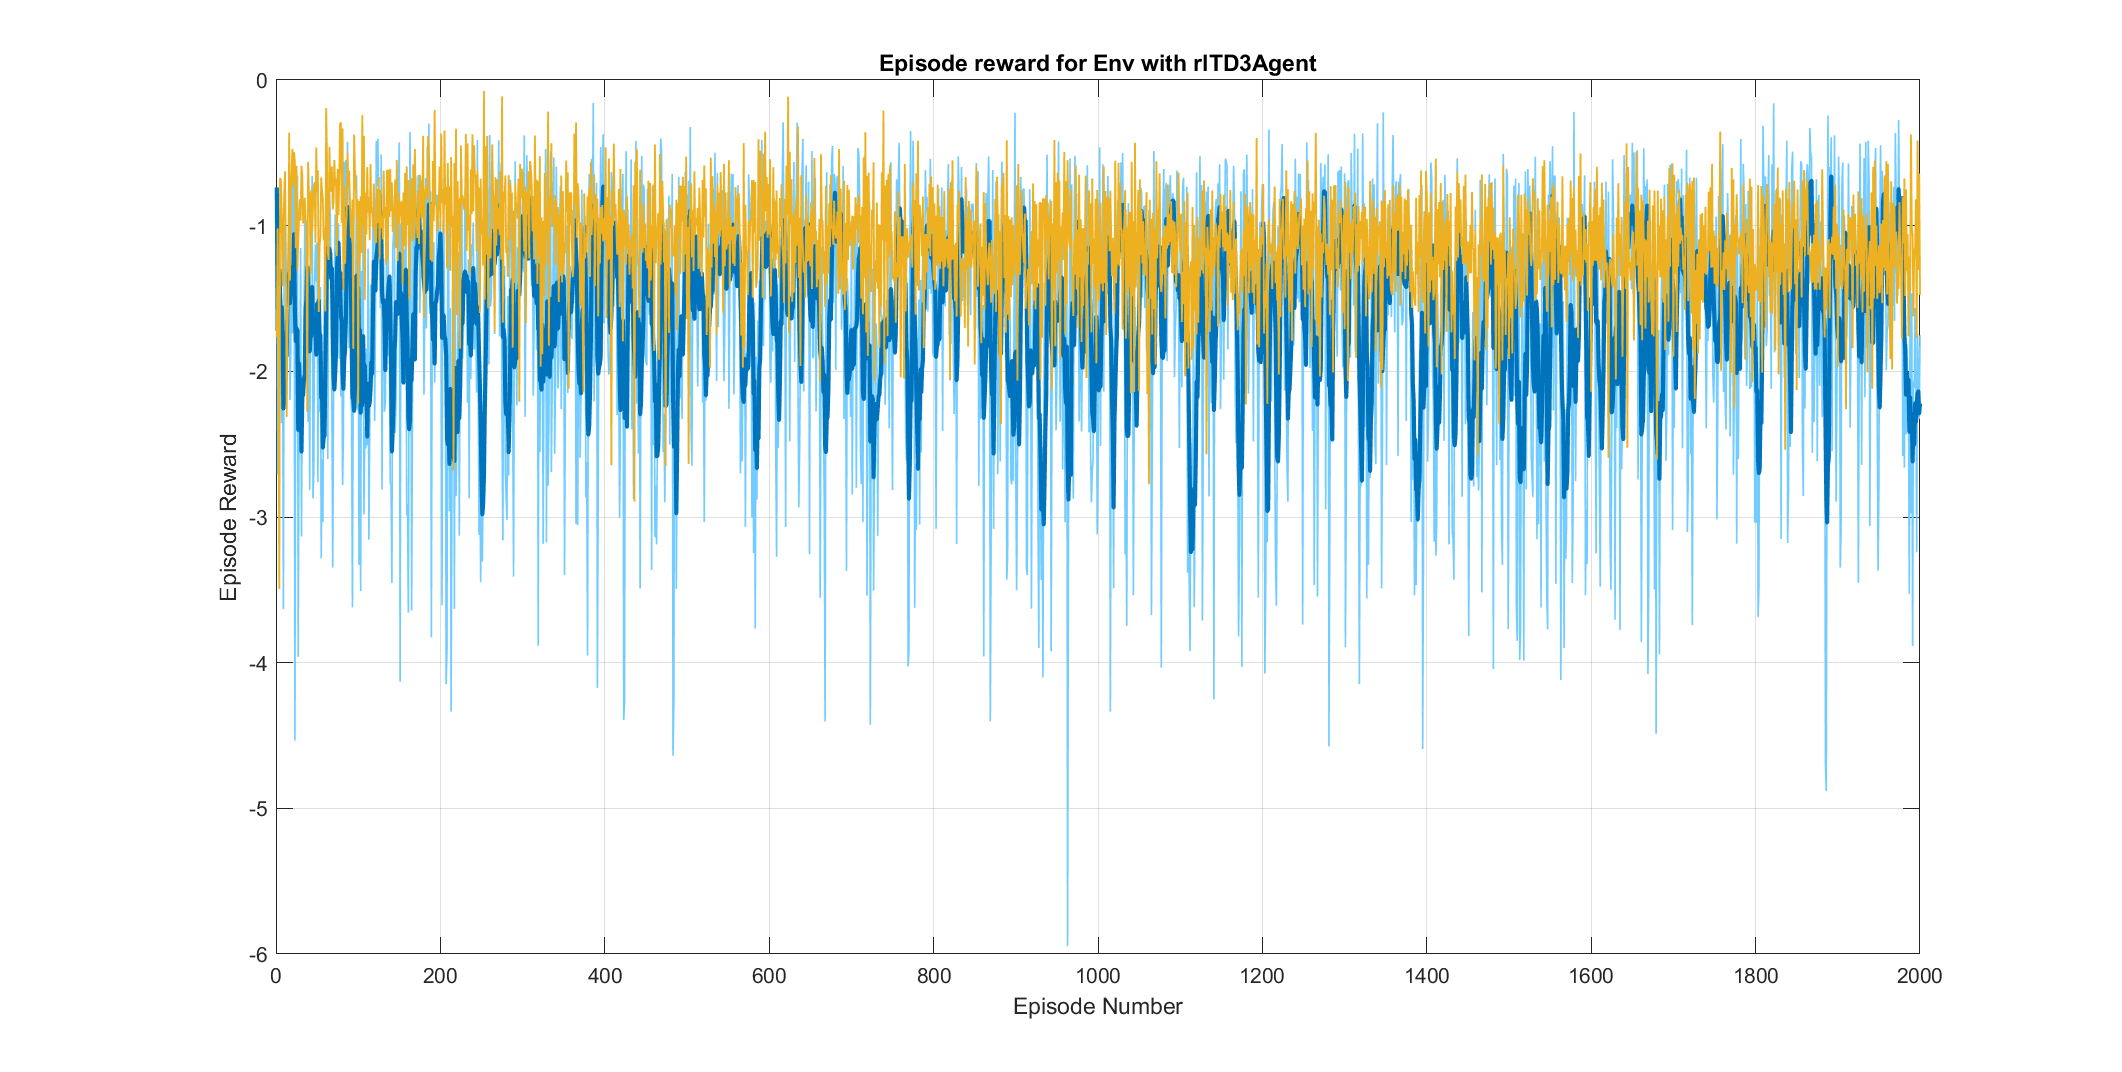
\includegraphics[width=\textwidth]{figures/training_progress_2000eps_markov.png}
\caption{Curva de entrenamiento de la intervenci\'on Markoviana de 2000 episodios.}
\label{fig:train2000}
\end{figure}
}{}

La corrida de 2000 episodios produjo las siguientes m\'etricas de entrenamiento:
\begin{itemize}[leftmargin=1.2cm]
    \item \texttt{EpisodeReward} medio: \(-1.6276\),
    \item \texttt{EpisodeReward} final: \(-1.7531\),
    \item mejor episodio: \(-0.1563\) en el episodio 386,
    \item \texttt{AverageReward} final: \(-2.2204\),
    \item mejor \texttt{AverageReward}: \(-0.6612\) en el episodio 1892,
    \item \texttt{EpisodeQ0} final: \(-1.4762\),
    \item pasos medios por episodio: \(14.54\),
    \item \texttt{trackingMSE} medio: \(0.10550\),
    \item \texttt{trackingMAE} medio: \(0.25861\),
    \item \texttt{actionL2} medio: \(0.33021\),
    \item \(|PWM|\) medio: \(128.29\),
    \item fracci\'on media de saturaci\'on: \(0.08478\),
    \item \(\Delta a\) L2 medio: \(0.28250\).
\end{itemize}

La comparaci\'on m\'as relevante ya no es contra la etapa \emph{legacy}, sino contra las dos etapas inmediatamente anteriores: \emph{remapeo 5000} y \emph{progreso+suavidad 3000}. La Tabla~\ref{tab:recent-train} resume esa comparaci\'on.

\begin{table}[H]
\centering
\caption{Comparaci\'on de corridas recientes de entrenamiento}
\label{tab:recent-train}
\footnotesize
\setlength{\tabcolsep}{4pt}
\renewcommand{\arraystretch}{1.15}
\resizebox{\textwidth}{!}{%
\begin{tabularx}{\textwidth}{L{0.17\textwidth}C{0.08\textwidth}C{0.10\textwidth}C{0.10\textwidth}C{0.10\textwidth}C{0.10\textwidth}C{0.10\textwidth}C{0.10\textwidth}C{0.10\textwidth}}
\toprule
\textbf{Configuraci\'on} & \textbf{\shortstack{Ep.}} & \textbf{\shortstack{MSE\\medio}} & \textbf{\shortstack{MAE\\medio}} & \textbf{\shortstack{Action\\L2}} & \textbf{\shortstack{|PWM|\\medio}} & \textbf{\shortstack{Frac.\\sat.}} & \textbf{\shortstack{\(\Delta a\)\\L2}} & \textbf{\shortstack{Reward\\media}} \\
\midrule
Remapeo & 5000 & 0.10701 & 0.26070 & 0.31081 & 125.06 & 0.05299 & 0.36496 & -1.5362 \\
Progreso+suavidad & 3000 & 0.10802 & 0.26197 & 0.25428 & 110.89 & 0.03969 & 0.36820 & -1.6005 \\
Markoviano + \(\Delta a\) observable & 2000 & 0.10550 & 0.25861 & 0.33021 & 128.29 & 0.08478 & 0.28250 & -1.6276 \\
\bottomrule
\end{tabularx}
}
\normalsize
\end{table}

La lectura correcta de esta tabla es la siguiente:
\begin{itemize}[leftmargin=1.2cm]
    \item el \texttt{trackingMSE} de entrenamiento baj\'o de \(0.10802\) a \(0.10550\) respecto a la etapa \emph{progreso+suavidad}, una mejora aproximada de \(2.3\%\);
    \item el \(\Delta a\) L2 medio baj\'o de \(0.36820\) a \(0.28250\), una reducci\'on aproximada de \(23.3\%\);
    \item pero el \texttt{actionL2} y la fracci\'on de saturaci\'on subieron en entrenamiento.
\end{itemize}

Esto ya anticipa una conclusi\'on importante: \textbf{la nueva intervenci\'on mejor\'o coordinaci\'on temporal y suavidad relativa entre acciones, pero no elimin\'o el uso de acci\'on fuerte ni la tendencia a saturar durante entrenamiento}. Tambi\'en es importante aclarar que los valores de reward entre configuraciones distintas no son estrictamente comparables, porque la reward cambi\'o entre etapas; por eso las m\'etricas prioritarias de comparaci\'on son \texttt{trackingMSE}, \texttt{trackingMAE}, \texttt{actionL2}, saturaci\'on y \(\Delta a\) L2.

\subsection{Test del \texttt{Agent2000}}

El test final del checkpoint \texttt{Agent2000} produjo:
\begin{itemize}[leftmargin=1.2cm]
    \item \texttt{trackingMSE} medio: \(0.10982\),
    \item \texttt{trackingMAE} medio: \(0.26389\),
    \item \texttt{actionL2} medio: \(0.28626\),
    \item \(|PWM|\) medio: \(118.55\),
    \item fracci\'on media de saturaci\'on: \(0.05786\),
    \item \(\Delta a\) L2 medio: \(0.18819\),
    \item reward media de test: \(-1.6890\),
    \item pasos medios por episodio: \(14.50\).
\end{itemize}

La comparaci\'on m\'as justa del test nuevo es contra el test de la etapa inmediatamente anterior, es decir, el test de \texttt{Agent3000} del experimento \emph{progreso+suavidad}. La Tabla~\ref{tab:test-compare} resume esa comparaci\'on.

\begin{table}[H]
\centering
\caption{Comparaci\'on de tests: etapa previa vs etapa Markoviana}
\label{tab:test-compare}
\footnotesize
\setlength{\tabcolsep}{5pt}
\renewcommand{\arraystretch}{1.15}
\resizebox{\textwidth}{!}{%
\begin{tabularx}{\textwidth}{L{0.28\textwidth}C{0.10\textwidth}C{0.10\textwidth}C{0.10\textwidth}C{0.10\textwidth}C{0.10\textwidth}C{0.10\textwidth}}
\toprule
\textbf{Checkpoint testeado} & \textbf{\shortstack{MSE\\medio}} & \textbf{\shortstack{MAE\\medio}} & \textbf{\shortstack{Action\\L2}} & \textbf{\shortstack{|PWM|\\medio}} & \textbf{\shortstack{Frac.\\sat.}} & \textbf{\shortstack{\(\Delta a\)\\L2}} \\
\midrule
Progreso+suavidad \texttt{Agent3000} & 0.10982 & 0.26389 & 0.42107 & 147.72 & 0.13485 & 0.52202 \\
Markoviano \texttt{Agent2000} & 0.10982 & 0.26389 & 0.28626 & 118.55 & 0.05786 & 0.18819 \\
\bottomrule
\end{tabularx}
}
\normalsize
\end{table}

Esta tabla es probablemente el resultado m\'as importante de toda la intervenci\'on nueva. La interpretaci\'on es muy clara:
\begin{itemize}[leftmargin=1.2cm]
    \item el \texttt{trackingMSE} de test no mejor\'o de forma apreciable;
    \item pero el \texttt{actionL2} cay\'o aproximadamente un \(32\%\);
    \item \(|PWM|\) medio cay\'o aproximadamente un \(19.7\%\);
    \item la fracci\'on de saturaci\'on cay\'o aproximadamente un \(57.1\%\);
    \item \(\Delta a\) L2 cay\'o aproximadamente un \(63.9\%\).
\end{itemize}

Es decir: la nueva formulaci\'on \textbf{no consigui\'o un mejor tracking final}, pero \textbf{s\'i produjo una pol\'itica mucho menos agresiva y mucho m\'as suave en evaluaci\'on}. Ese resultado es relevante porque corrige justamente uno de los defectos dominantes de la etapa anterior: una pol\'itica con tracking parecido, pero demasiado costosa y saturada.

\subsection{Lectura visual del test}

\IfFileExists{figures/test_episode_49_3000.png}{
\IfFileExists{figures/test_episode_49_markovian.png}{
\begin{figure}[H]
\centering
\begin{minipage}{0.49\textwidth}
\centering
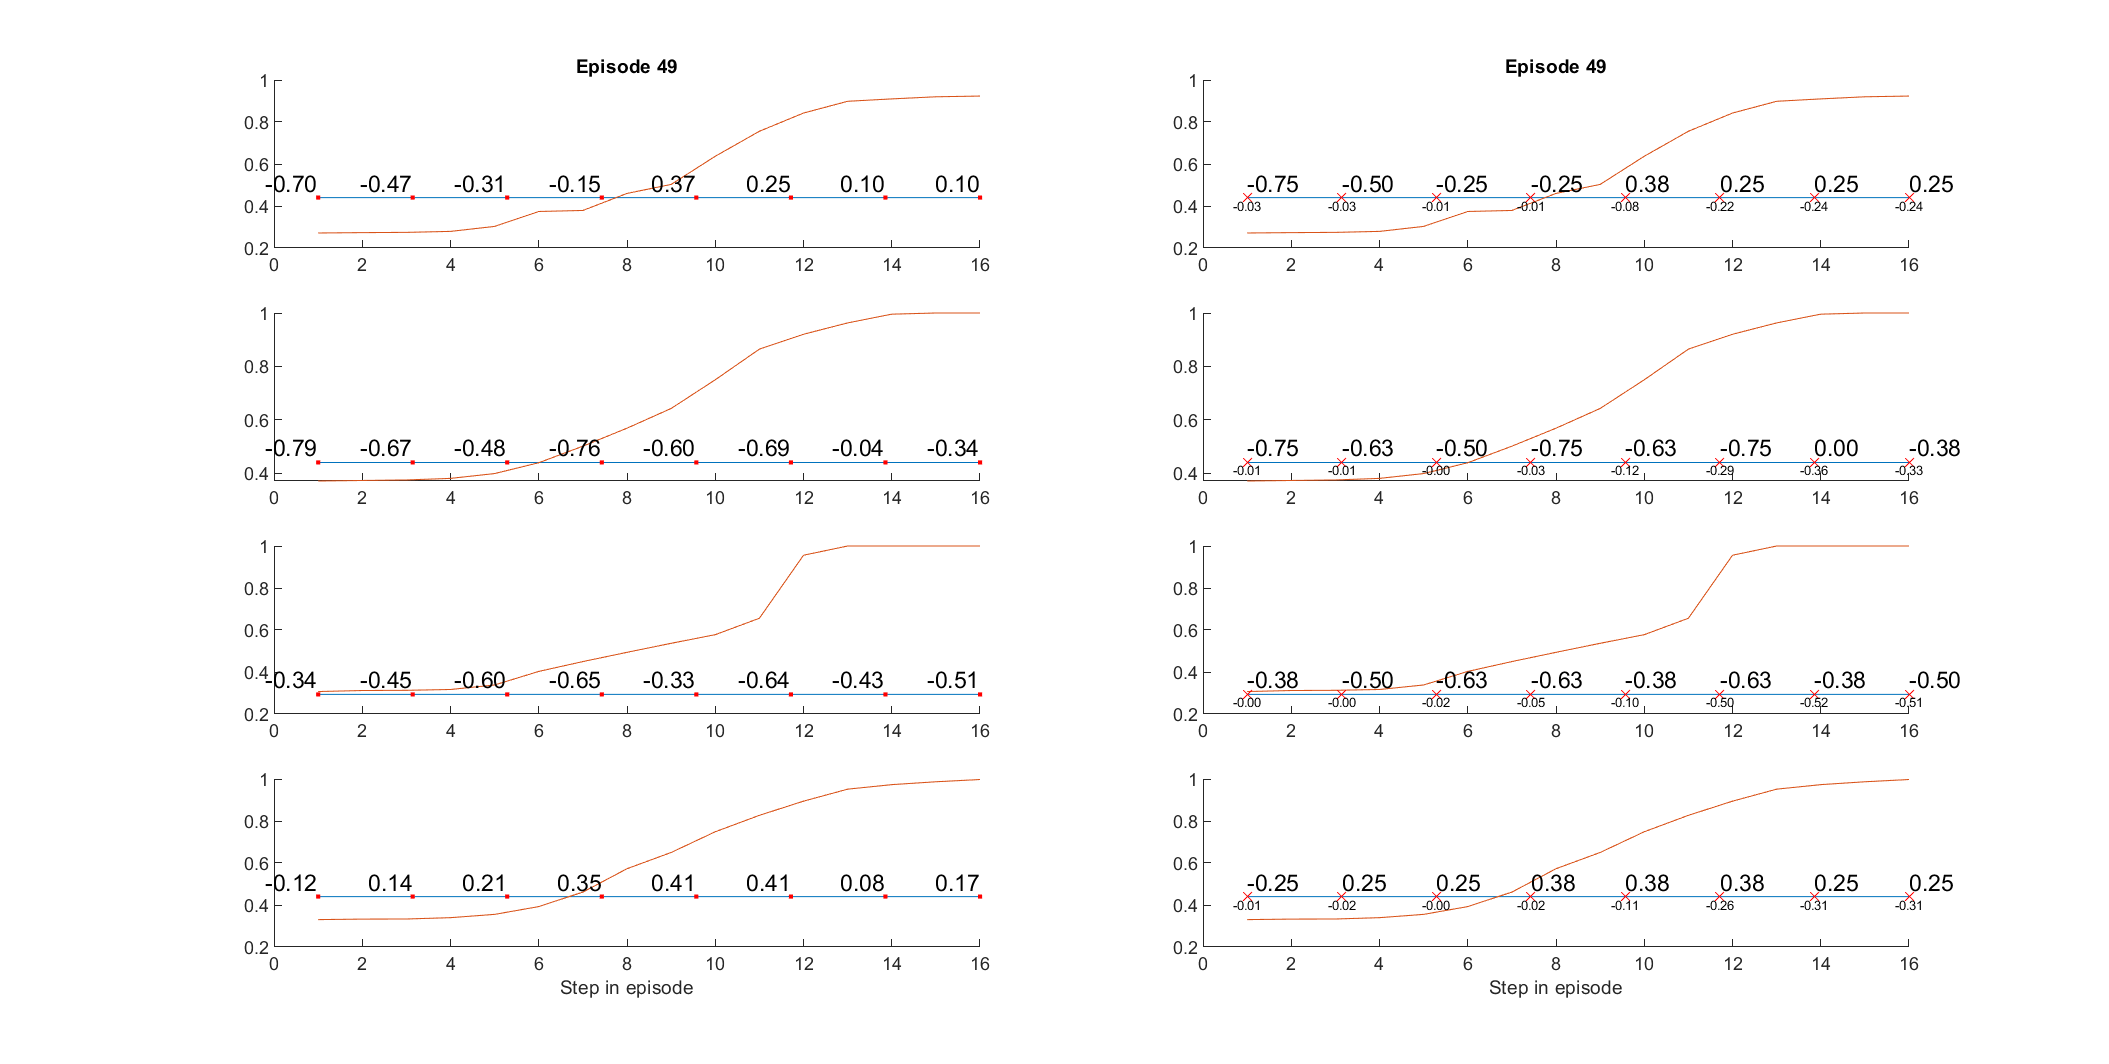
\includegraphics[width=\textwidth]{figures/test_episode_49_3000.png}
\caption*{(a) Etapa progreso+suavidad, \texttt{Agent3000}}
\end{minipage}
\hfill
\begin{minipage}{0.49\textwidth}
\centering
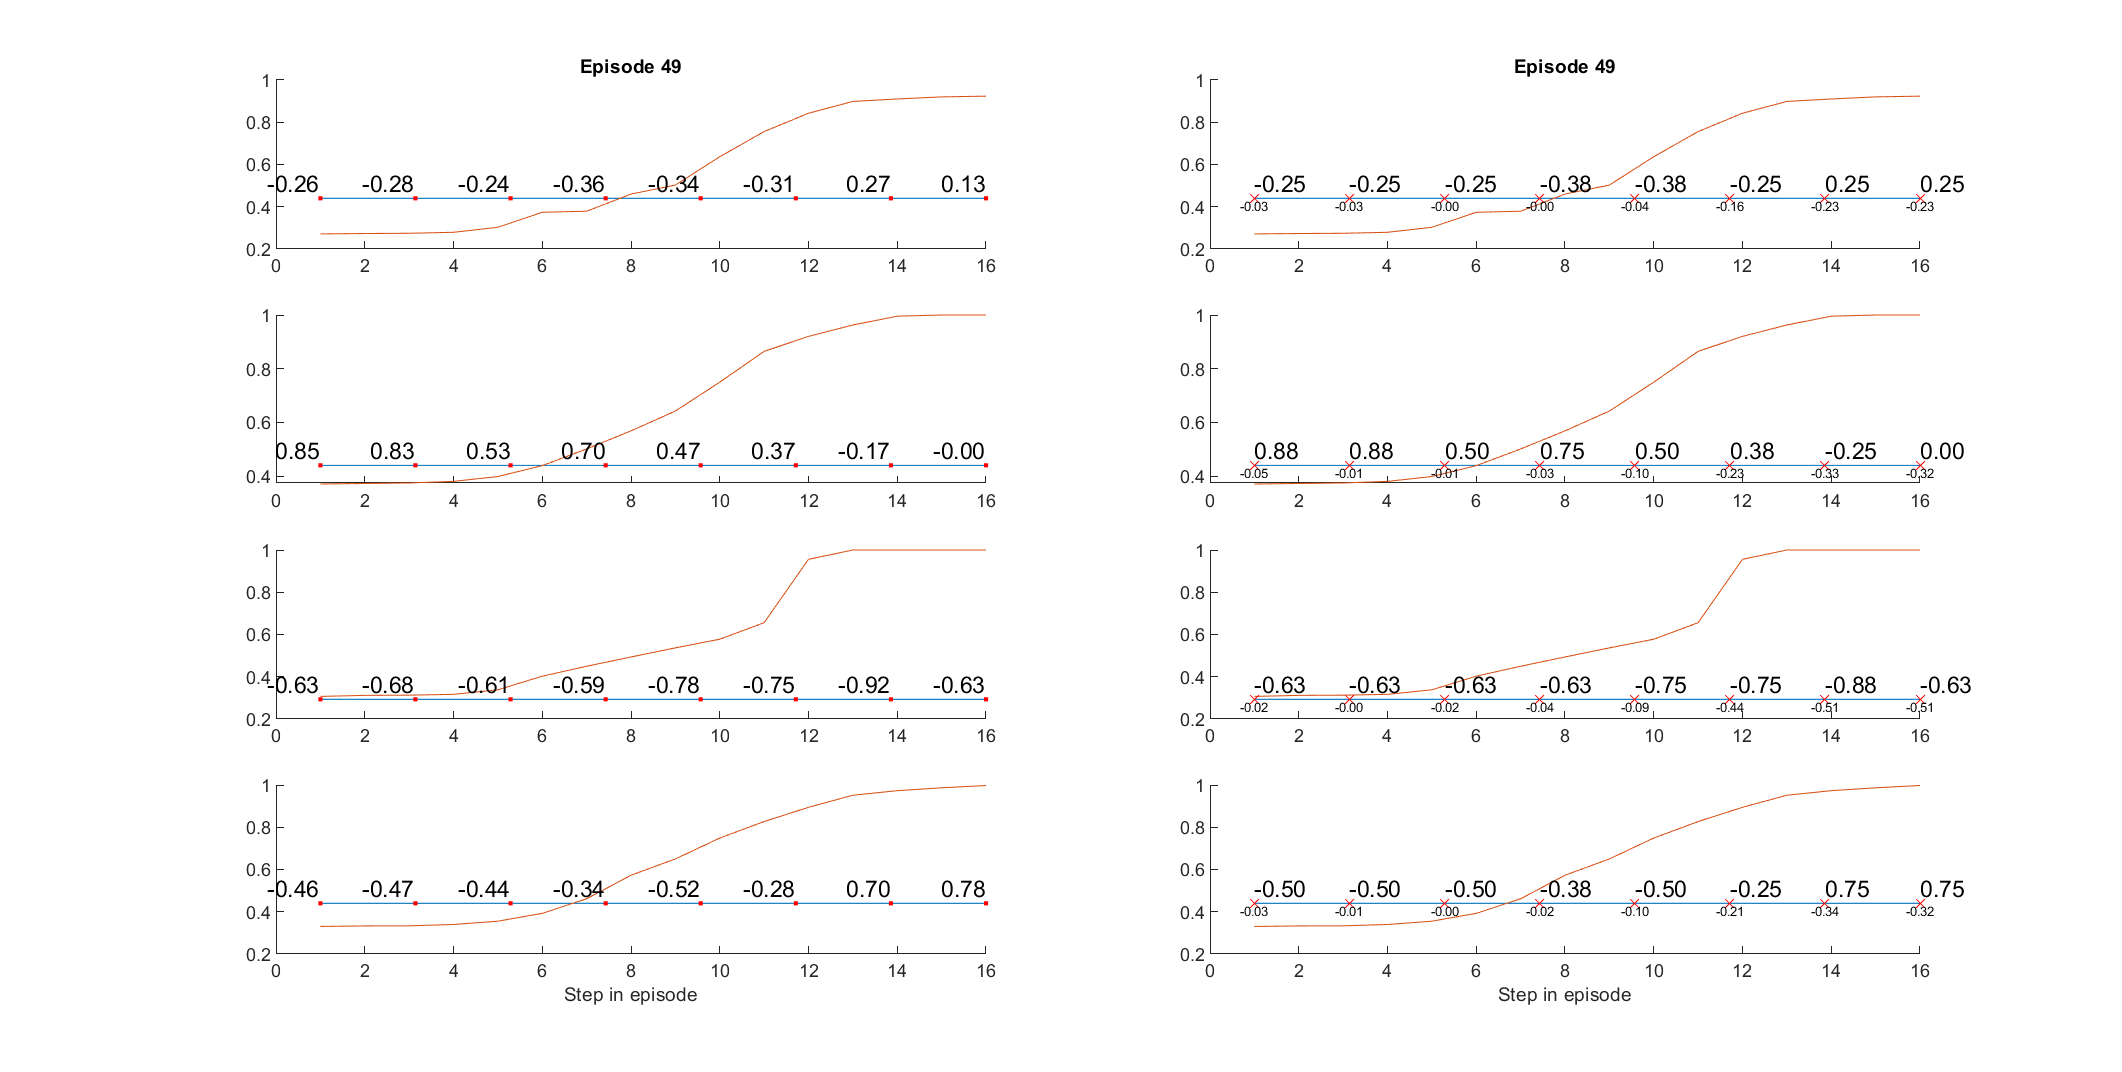
\includegraphics[width=\textwidth]{figures/test_episode_49_markovian.png}
\caption*{(b) Etapa Markoviana, \texttt{Agent2000}}
\end{minipage}
\caption{Comparaci\'on visual del episodio 49 en test. La salida azul sigue lejos de la referencia naranja en ambos casos, pero la pol\'itica nueva muestra acciones menos extremas y menor saturaci\'on visible.}
\label{fig:testcompare}
\end{figure}
}{}
}{}

La Figura~\ref{fig:testcompare} confirma visualmente lo que ya mostraban las m\'etricas:
\begin{itemize}[leftmargin=1.2cm]
    \item la pr\'otesis sigue sin seguir de forma satisfactoria la trayectoria naranja de referencia;
    \item por tanto, el problema de tracking persiste;
    \item sin embargo, la pol\'itica nueva no est\'a colapsando al mismo nivel de control agresivo que la etapa previa.
\end{itemize}

En el episodio 49 del test Markoviano, las acciones efectivas se observan m\'as moduladas por canal. Todav\'ia aparecen signos mixtos y tramos de acci\'on relativamente grandes, pero el patr\'on es menos cercano a un \emph{bang-bang} saturado sostenido. La lectura cualitativa coincide con la cuantitativa: \textbf{se mejor\'o calidad de control, no tracking}.

\section{Interpretaci\'on t\'ecnica}

La conclusi\'on t\'ecnica m\'as importante de esta etapa es que la intervenci\'on nueva \textbf{s\'i resolvi\'o un problema de dise\~no del experimento}. La reward ya no depende de historia oculta y el actor ya observa la informaci\'on temporal m\'inima relevante. Eso hace al sistema m\'as coherente desde el punto de vista de RL y m\'as defendible desde el punto de vista metodol\'ogico.

Sin embargo, el resultado tambi\'en deja claro que el cuello de botella actual cambi\'o de naturaleza:
\begin{enumerate}[leftmargin=1.2cm]
    \item ya no es la falta de acci\'on efectiva;
    \item ya no es una reward mal formulada en lo b\'asico;
    \item ahora el problema dominante es la \textbf{capacidad de la pol\'itica para traducir EMG instant\'aneo en coordinaci\'on multi-canal fina}.
\end{enumerate}

La evidencia concreta que sostiene esa interpretaci\'on es:
\begin{itemize}[leftmargin=1.2cm]
    \item el \texttt{trackingMSE} de test qued\'o pr\'acticamente igual entre la etapa previa y la actual;
    \item la nueva etapa s\'i redujo fuertemente saturaci\'on, PWM medio y cambio de acci\'on;
    \item por tanto, el nuevo dise\~no no empeor\'o el tracking, pero tampoco consigui\'o extraer mejor informaci\'on de la EMG para seguir la referencia.
\end{itemize}

Desde un punto de vista experimental, eso es un hallazgo valioso. No es un fracaso del cambio: es una delimitaci\'on mucho m\'as clara del problema real. El proyecto pas\'o de un escenario donde el agente estaba sesgado por reward y por actuaci\'on no f\'isica a un escenario donde la pol\'itica ya es m\'as suave y coherente, pero la representaci\'on disponible sigue siendo insuficiente para tracking fino.

\section{Veredicto actual}

El veredicto de esta etapa es el siguiente:
\begin{itemize}[leftmargin=1.2cm]
    \item \textbf{S\'i conviene mantener} el estado ampliado de 52 dimensiones.
    \item \textbf{S\'i conviene mantener} la reward simplificada sin t\'ermino de progreso oculto.
    \item \textbf{S\'i conviene mantener} el remapeo a acci\'on efectiva.
    \item \textbf{No conviene todav\'ia} pasar a hardware.
    \item \textbf{No conviene} interpretar este resultado como un problema puramente de ``m\'as episodios''.
\end{itemize}

La etapa Markoviana dej\'o una mejora cualitativa real en la pol\'itica: menor saturaci\'on, menor esfuerzo y mucha menor variaci\'on entre acciones. Eso es importante. Pero el resultado tambi\'en deja una conclusi\'on inequ\'ivoca: \textbf{todav\'ia no existe una mejora suficiente de tracking para considerar la tarea resuelta}.

\section{Trabajo futuro recomendado}

Con base en estas evidencias, el siguiente trabajo recomendado es:
\begin{enumerate}[leftmargin=1.2cm]
    \item \textbf{Auditor\'ia de checkpoints de la corrida Markoviana.}\\
    El mejor \texttt{AverageReward} ocurri\'o cerca del episodio 1892. La evaluaci\'on del \texttt{Agent2000} fue necesaria para cerrar la corrida, pero lo correcto ahora es auditar checkpoints cercanos (\texttt{Agent1800}, \texttt{Agent1850}, \texttt{Agent1900}, \texttt{Agent1950}, \texttt{Agent2000}) antes de decidir si esta intervenci\'on ya dio su mejor pol\'itica.

    \item \textbf{Aumentar contexto temporal EMG antes de cambiar algoritmo.}\\
    La nueva intervenci\'on solo a\~nadi\'o memoria m\'inima de encoders y acci\'on previa. El siguiente cambio de menor riesgo no es SAC ni LSTM directo, sino enriquecer el contexto temporal de entrada conservando TD3. Eso podr\'ia hacerse con apilado corto de ventanas EMG o con features temporales adicionales, porque la literatura de control mioel\'ectrico enfatiza precisamente la relevancia de la estructura temporal \citep{chen2023review}.

    \item \textbf{Mantener la comparaci\'on en simulaci\'on pura.}\\
    Antes de considerar hardware, la siguiente iteraci\'on debe demostrar o bien una reducci\'on visible de \texttt{trackingMSE}, o bien una mejora equivalente en tracking sin perder la suavidad conseguida ahora.

    \item \textbf{Mantener como rama futura la acci\'on h\'ibrida.}\\
    Dado que el actuador real aplica niveles cuantizados y no una acci\'on verdaderamente continua, una futura l\'inea de investigaci\'on podr\'ia explorar representaciones h\'ibridas de acci\'on, como las propuestas en HyAR \citep{li2021hyar}. Esa idea tiene fundamento, pero todav\'ia no es el cambio de menor riesgo en esta etapa.
\end{enumerate}

\section{Conclusi\'on}

La intervenci\'on Markoviana fue \textbf{correcta y necesaria}. Mejor\'o la consistencia del problema para TD3, elimin\'o historia oculta de la reward y produjo una pol\'itica de evaluaci\'on notablemente m\'as suave. El resultado cuantitativo m\'as importante es que esa mejora de suavidad no vino acompa\~nada de una penalizaci\'on fuerte en tracking; el \texttt{trackingMSE} de test qued\'o esencialmente igual mientras el costo de control cay\'o de forma marcada.

No obstante, la meta del proyecto sigue siendo seguimiento satisfactorio de la intenci\'on motora, no solo suavidad. Por eso el balance final de esta etapa es mixto: \textbf{avance metodol\'ogico claro, mejora de calidad de control clara, mejora de tracking final todav\'ia insuficiente}. Esa es precisamente la informaci\'on que se necesitaba para orientar la siguiente iteraci\'on con criterio t\'ecnico y sin pasar prematuramente a hardware.

\bibliographystyle{plainnat}
\bibliography{references}

\end{document}
